\documentclass[a4paper,oneside]{scrarticle}

\usepackage[left=3cm,right=3cm,top=2cm,bottom=2.25cm]{geometry}
\usepackage[ngerman]{babel}
\usepackage{amsmath}
\usepackage{amsfonts}
\usepackage{amssymb}
\usepackage{mathtools}
\usepackage{graphicx}
%\graphicspath{ {./images/} }
\addto\captionsngerman{\renewcommand{\figurename}{Fig.}}


\begin{document}
	\begin{flushleft}
		Bach Nguyen, Johannes Roloff - HTWK Leipzig - INB
	\end{flushleft}
	\begin{center}
		\begin{LARGE}
			\textbf{Station 5 Evaluation}
		\end{LARGE}
	\end{center}
	\section*{Einordnung der Aufgabe im Prozess}
	\begin{figure} [h]
		\centering
		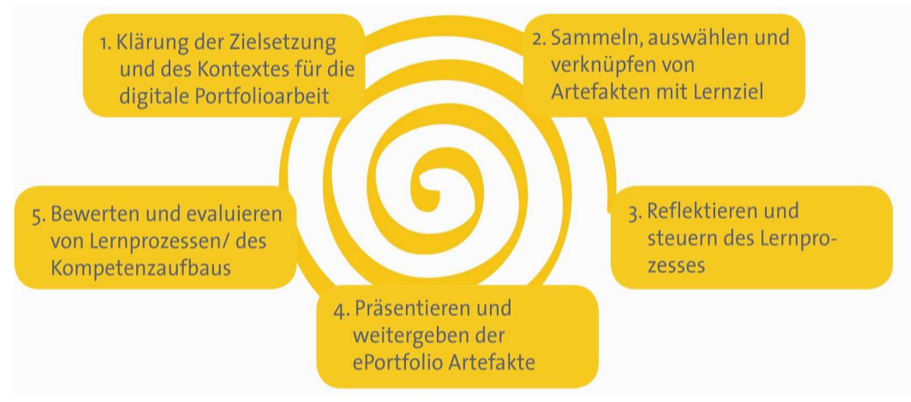
\includegraphics[width=0.7\linewidth]{e-portfolio-prozesse-schaffert}
		\caption{E-unterstützte Portfolio Prozesse (Schaffert et al. 2007)}
		\label{fig:e-portfolio-prozesse-schaffert}
	\end{figure}
	\begin{figure}[h]
		\centering
		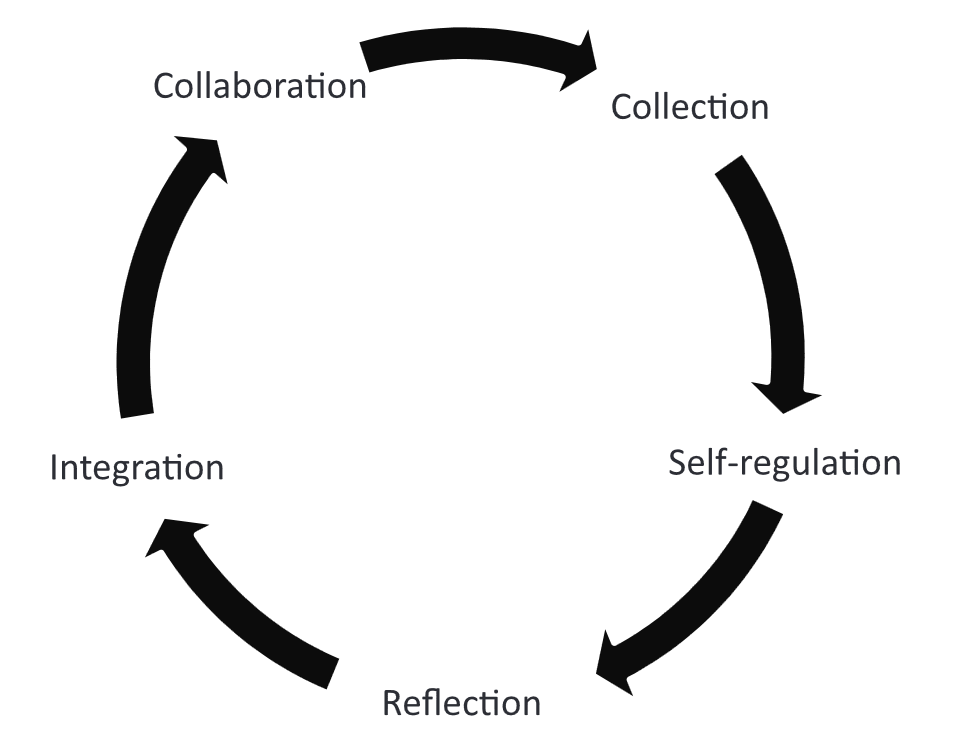
\includegraphics[width=0.7\linewidth]{cycle-of-documented-lifelong-learning-Jensen}
		\caption{cycle of documented lifelong learning (Jensen,Treuer 2014)}
		\label{fig:cycle-of-documented-lifelong-learning-jensen}
	\end{figure}
	\pagebreak 
	
	\section*{Einleitung}
	An dieser Stelle beginnt die Evaluationsphase. Bewerte Deinen eigenen Lernfortschritt. Dies ist eine weiterführende Art der Reflexion. 
	
	\section*{Aufgabenstellung}

	\begin{enumerate}
		\item Schaue zuerst zurück auf das ausgewählte Modul. Schreibe einen Evaluationsbericht über deinen Lernfortschritt. Nutze dazu Modulux und beantworte, ob du die Lernziele erreicht hast. Beantworte ebenfalls folgende Fragen.
		\begin{enumerate}
			\item Spiegelt sich mein Gelerntes in meiner Note wieder?
			\item 
		\end{enumerate}
		\item Für dein Studium, sammle aus mindestens 3 Modulen jeweils deine bestes Werk
		\begin{enumerate}
			\item Was war mein Anteil bei dieser Aufgabe?
			\item Was habe ich gelernt?
			\item Wie hat dies andere Menschen oder Dinge positiv beeinflusst?
		\end{enumerate}

	\end{enumerate}


\end{document}
